\subsection{Dissimilarity metrics}

The reconstruction of the puzzle is based on a dissimilarity metric between all the pieces. The higher the dissimilarity between two given pieces, the lower priority is given to the fact that these pieces are placed next to each other. Several dissimilarity metrics are introduced.

\autoref{fig:side} depicts the working principle of the dissimilarity computation. The intensity of the red channel for the right side of a piece of the puzzle is plotted along with the left side of two others pieces. One can see that the matching piece has nearly the same profile as the starting piece (nearly superimposed), while the third one is very different. Of course, the difference between matching and non matching pieces are not always that obvious.

\begin{figure}[H]
    \centering
    % This file was created by matlab2tikz.
%
%The latest updates can be retrieved from
%  http://www.mathworks.com/matlabcentral/fileexchange/22022-matlab2tikz-matlab2tikz
%where you can also make suggestions and rate matlab2tikz.
%
\definecolor{mycolor1}{rgb}{0.00000,0.44700,0.74100}%
\definecolor{mycolor2}{rgb}{0.85000,0.32500,0.09800}%
\definecolor{mycolor3}{rgb}{0.92900,0.69400,0.12500}%
%
\begin{tikzpicture}

\begin{axis}[%
width=.8\linewidth,
height=.3\textheight,
at={(0.758in,0.481in)},
scale only axis,
xmin=0,
xlabel=Y coordinate,
ylabel= Red intensity,
xmax=60,
ymin=0.2,
ymax=1,
axis background/.style={fill=white},
legend style={legend cell align=left, align=left, draw=white!15!black},
cycle list name=exotic
]
\addplot +[mark=*]
  table[row sep=crcr]{%
1	0.971252002746624\\
2	0.948149843595026\\
3	0.968062867170211\\
4	0.958236057068738\\
5	0.903639276722359\\
6	0.767345693141067\\
7	0.64028381780728\\
8	0.697657740138858\\
9	0.860761425192642\\
10	0.890989547570001\\
11	0.761669336995496\\
12	0.684290836957352\\
13	0.629907682917526\\
14	0.607110704203862\\
15	0.56993972686351\\
16	0.52587167162585\\
17	0.518013275349048\\
18	0.529381246662091\\
19	0.704005493247884\\
20	0.574456397344932\\
21	0.621713588158997\\
23	0.614282444495309\\
24	0.68157473105974\\
25	0.595407034409092\\
26	0.569604028381782\\
27	0.566186007476922\\
28	0.560372320134277\\
29	0.568352788586253\\
30	0.591973754482339\\
31	0.610605020218202\\
32	0.604638742656597\\
33	0.727504386968796\\
34	0.844251163500417\\
35	0.749416342412452\\
36	0.663630121309225\\
37	0.496574349584193\\
38	0.477454795147629\\
39	0.476050965133133\\
40	0.465796902418553\\
41	0.469260700389107\\
42	0.583916990920883\\
43	0.585259784847793\\
44	0.456076905470361\\
45	0.449423971923402\\
46	0.437735561150532\\
47	0.441870756084533\\
48	0.439841306172276\\
49	0.442847333485922\\
50	0.454322117952238\\
51	0.467017624170289\\
52	0.454596780346378\\
53	0.443945983062484\\
54	0.430884260318912\\
55	0.420675974670026\\
56	0.402288853284503\\
};
\addlegendentry{Right of start piece}

\addplot +[mark=square]
  table[row sep=crcr]{%
1	0.286991683833065\\
2	0.274052033264667\\
3	0.288242923628594\\
4	0.295414663920042\\
5	0.288944838635842\\
6	0.270939192797741\\
7	0.275501640344856\\
8	0.274525062943468\\
9	0.436392767223623\\
10	0.449271381704435\\
11	0.336079957274741\\
12	0.324773022049285\\
13	0.385030899519343\\
14	0.39407949950408\\
15	0.360646982528422\\
16	0.352040894178685\\
17	0.367254139009688\\
18	0.401327534905015\\
19	0.422247653925382\\
20	0.393194476234072\\
21	0.386633096818493\\
22	0.398550392919816\\
23	0.371541924162663\\
24	0.308812085145341\\
25	0.305653467612728\\
26	0.307240405889985\\
27	0.302754253452356\\
28	0.317112993057144\\
29	0.320943007553218\\
30	0.36107423514153\\
31	0.452903028915848\\
32	0.527611200122074\\
33	0.548821240558482\\
34	0.553612573434044\\
35	0.528542000457769\\
36	0.494453345540549\\
37	0.48476386663615\\
38	0.573678187228197\\
39	0.516609445334552\\
40	0.461478599221792\\
41	0.43123521782254\\
42	0.440665293354698\\
43	0.39049362935836\\
44	0.213794155794616\\
45	0.221118486305031\\
46	0.279621576256964\\
47	0.285420004577709\\
48	0.302006561379415\\
49	0.355062180514231\\
50	0.411276417181661\\
51	0.47081712062257\\
52	0.479209582665753\\
53	0.506279087510492\\
54	0.480277714198522\\
55	0.465644312199586\\
56	0.478629739833679\\
};
\addlegendentry{Left of not matching piece}


\addplot +[mark=x]
  table[row sep=crcr]{%
1	0.967650873579004\\
2	0.94709697108415\\
3	0.96752880140383\\
4	0.966613260090028\\
5	0.897413595788507\\
6	0.750087739375907\\
7	0.639963378347446\\
8	0.701304646372165\\
9	0.866834515907527\\
10	0.886289768825819\\
11	0.771496147096968\\
12	0.696345464255742\\
13	0.62345311665522\\
14	0.590737773708703\\
15	0.547173266193639\\
16	0.542412451361869\\
17	0.514351110093841\\
18	0.521660181582362\\
19	0.700053406576636\\
20	0.570931563286791\\
21	0.605630579079879\\
22	0.618509193560691\\
23	0.615793087663079\\
24	0.684412909132526\\
25	0.60106813153277\\
26	0.562188143739988\\
27	0.561013199053939\\
28	0.550896467536433\\
29	0.562294956893261\\
30	0.582482642862594\\
31	0.605493247882812\\
32	0.586511024643322\\
33	0.703715571831843\\
34	0.855069810025178\\
35	0.756343938353552\\
36	0.678278782330054\\
37	0.494071869993135\\
38	0.478233005264364\\
39	0.470160982681008\\
40	0.466392004272528\\
41	0.473197528038455\\
42	0.563912413214311\\
43	0.59746700236515\\
44	0.458899824521247\\
45	0.447211413748377\\
46	0.438376440070193\\
47	0.43842221713588\\
48	0.441824979018847\\
49	0.443823910887311\\
50	0.453971160448617\\
51	0.469993133440148\\
52	0.463050278477148\\
53	0.444510566872665\\
54	0.420737010757612\\
55	0.423895628290225\\
56	0.40064087891966\\
};
\addlegendentry{Left of matching piece}


\end{axis}
\end{tikzpicture}%
    \caption{Illustration of the principle of dissimilarity computation by showing the red channel intensities for three pieces.}
    \label{fig:side}
\end{figure}

\paragraph{Sum of Squared Distances (SSD)} \mbox{} 

The SSD between two pieces $x_i$ and $x_j$ is obtained by summing up the squared differences of the pixels along the pieces' juxtaposing boundaries, for each color channel (red, green and blue) \cite{robust}. For a piece $x$ of size $M \times M$, $x(m,n,c)$ denotes the value of the pixel at the coordinates $(m,n)$ in the color channel $c$. The SSD between $x_i$ and $x_j$, $x_i$ being placed at the left of $x_j$, can be expressed as 

\begin{equation}
    D_{LR,SSD}(x_i, x_j) = \sum_{c=1}^{3} \sum_{k=1}^{M} \left( x_i(k,M,c) - x_j(k,M,c)\right)^2    
\end{equation}

This can be extended to the cases where $x_i$ is placed on the right, on the top or on the bottom of $x_j$.

\paragraph{$(L_p)^q$ norm} \mbox{}

The SSD is actually the $L_2$ norm of the two vectors that form the boundaries of the two pieces. The $(L_p)^q$ can also be used, and it is defind as

\begin{equation}\label{eq:lpq}
    \hspace{-0.3cm}
    D_{LR,pq}(x_i, x_j) = \left( \sum_{c=1}^{3} \sum_{k=1}^{M} \left( \left| x_i(k,M,c) - x_j(k,M,c)\right|\right)^p \right)^{\frac{p}{q}}
\end{equation}

Hence, the SSD is a particular case of $(L_p)^q$ norm with $p=q=2$. It was experimentally found in \cite{greedy} that the good results were obtained for $p=3/10$ and $q=1/16$, they will thus be used in the solver. Instinctively, it is due to the fact that the $L_2$ norm penalizes a lot large boundary differences even though such differences may occur in natural images. 

\paragraph{Mahalanobis Gradient Compatibility (MGC)}

While the first two metrics penalize differences in the pixels intensities, the MGC (introduced in \cite{Gallagher}) instead penalizes differences in the intensity of the gradient. If a piece has a strong gradient near its edge, it is expected that the juxtaposed piece will continue the gradient. The penalty for a deviation is computed with the Mahalanobis distance.

Looking at the dissimilarity between the right side of $x_i$ and the left side of $x_j$, let $\mu_{iL}(c)$ be the average color difference in the color channel $c$ between the two last columns of $x_i$:

\begin{equation}
    \mu_{iL}(c) = \frac{1}{M} \sum_{k=1}^{M} x_i(k,M,c) - x_i(k,M-1,c) 
\end{equation}

The array of gradients of dimension $M$ by 3 $G_{ijLR}$ is then introduced, with $G_{ijLR}(k,c)$ denoting the color difference between the right side of $x_i$ and the left side of $x_j$ for the color channel $c$ at the row $k$:

\begin{equation}
    G_{ijLR}(k,c) = x_j(k,1,c) - x_i(k,M,c) 
\end{equation}

By denoting $S_{iL}$ the 3 by 3 covariance matrix obtained from the gradient difference at the right of $x_i$, the gradient dissimilarity is given by:

\begin{gather}
    D'_{LR}(x_i,x_j) = \sum_{k=1}^{M} D'_{LR,k}\\
    D'_{LR,k} = \left( G_{ijLR}(k) - \mu_{iL} \right) S_{iL}^{-1} \left( G_{ijLR}(k) - \mu_{iL} \right)^T
\end{gather}

The final MGC symmetric dissimilarity metric for placing the piece $x_i$ at the left of $x_j$ is given by:

\begin{equation}
    D_{LR,MGC}(x_i,x_j) = D'_{LR}(x_i,x_j) +  D'_{RL}(x_j,x_i)
\end{equation}

\paragraph{Combining MGC and SSD (M+S)} \mbox{}

It was proposed in \cite{robust} that the SSD and the MGC convey complementary information so that they could be combined to provide more accuracy. The M+S dissimilarity metric is hence defined as the weighed product of the SSD and the MGC:

\begin{equation}\label{eq:ms}
    D_{M+S}(x_i,x_j) = D_{MGC}(x_i,x_j) \times \left( D_{SSD}(x_i,x_j) \right)^{\frac{1}{r}}
\end{equation}

The value of the weighing parameter $r$ giving the best results is investigated later.

%The obtained dissimilarities are then normalized \cite{robust} \cite{Gallagher}. For a given piece, all its dissimilarities are divided by the 

\paragraph{Combining MGC and $(L_p)^q$ (M+pq)} \mbox{}

In the same idea, the MGC and the $(L_p)^q$ can be combined in a weighed product. This method will be referred to as the M+pq in the latter.

\begin{equation}\label{eq:mpq}
    D_{M+pq}(x_i,x_j) = D_{MGC}(x_i,x_j) \times \left( D_{pq}(x_i,x_j) \right)^{\frac{1}{r}}
\end{equation}

\subsection{Placement algorithm}

Once the dissimilarity is evaluated between every piece of the puzzle, for every orientation (top, bottom, right, left), the pieces should be placed accordingly to these measures. The implemented algorithm is a two step iterative method, and it is inspired from what was proposed in \cite{greedy}. An illustration of its functioning is depicted in \autoref{fig:placement}.

The starting piece is chosen to be the one having the lowest dissimilarity with any other piece of the puzzle. During the first step, all the pieces that have already been placed are scanned. The next piece that will be placed on the puzzle  is the one that has the lowest dissimilarity with any of the already placed ones. Piece by piece, the puzzle is then reconstructed. When a piece has to be placed in between multiple others, the dissimilarity with all of these is taken into account.


The second step starts when the puzzle is full. The algorithm then looks for \textit{symmetric matches} in all the juxtaposed pieces. Two pieces $x_i$ and $x_j$ are symmetrically matched if the best possible match for $x_i$ in every possible orientation is $x_j$ and the best possible match for $x_j$ is $x_i$ in the opposite orientation. For example, if the pieces labeled $x_3$ and $x_7$ are juxtaposed at the end of the first step, they will be considered as symmetric matches if the best possible match for $x_3$ is $x_7$ on its right, and the best match for $x_7$ is $x_3$ on its left. From these symmetric matches, a \textit{segment} is extracted from the image. It is defined as the biggest portion of the puzzle only composed of symmetrically matched pieces, and will serve as starting point for the next iteration. The iteration process stops when the result after the reconstruction step is not changing anymore.

\begin{figure}[H]
    \centering
%     \subfloat[The puzzle is constructed piece by piece.]{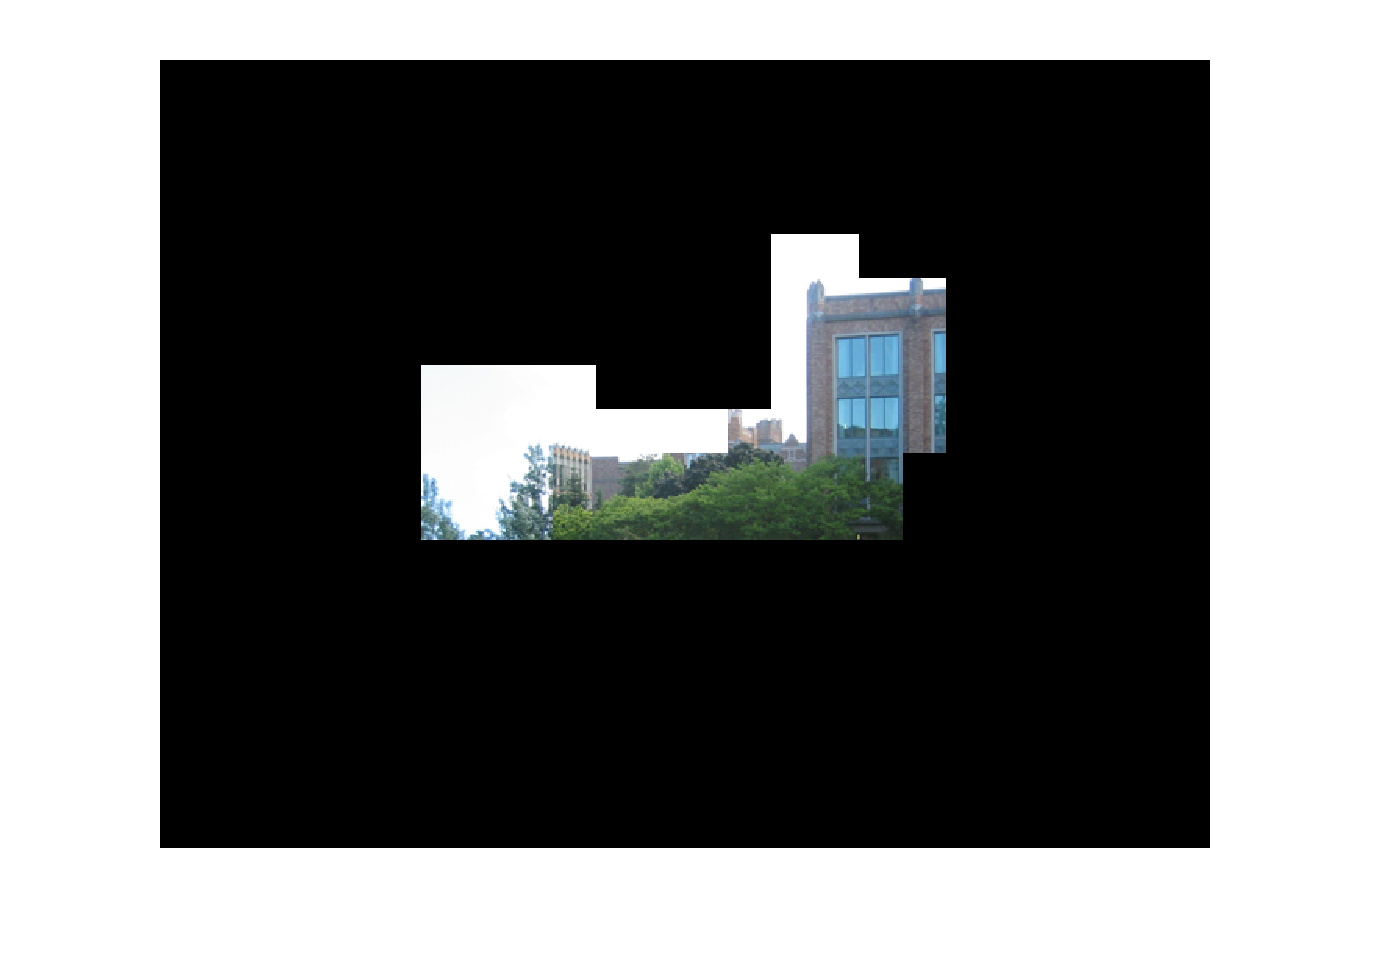
\includegraphics[height=0.25\textheight]{fig/algo_start.eps}
% \label{fig:placement1}}
% \hfil
%     \subfloat[The puzzle is constructed piece by piece.]{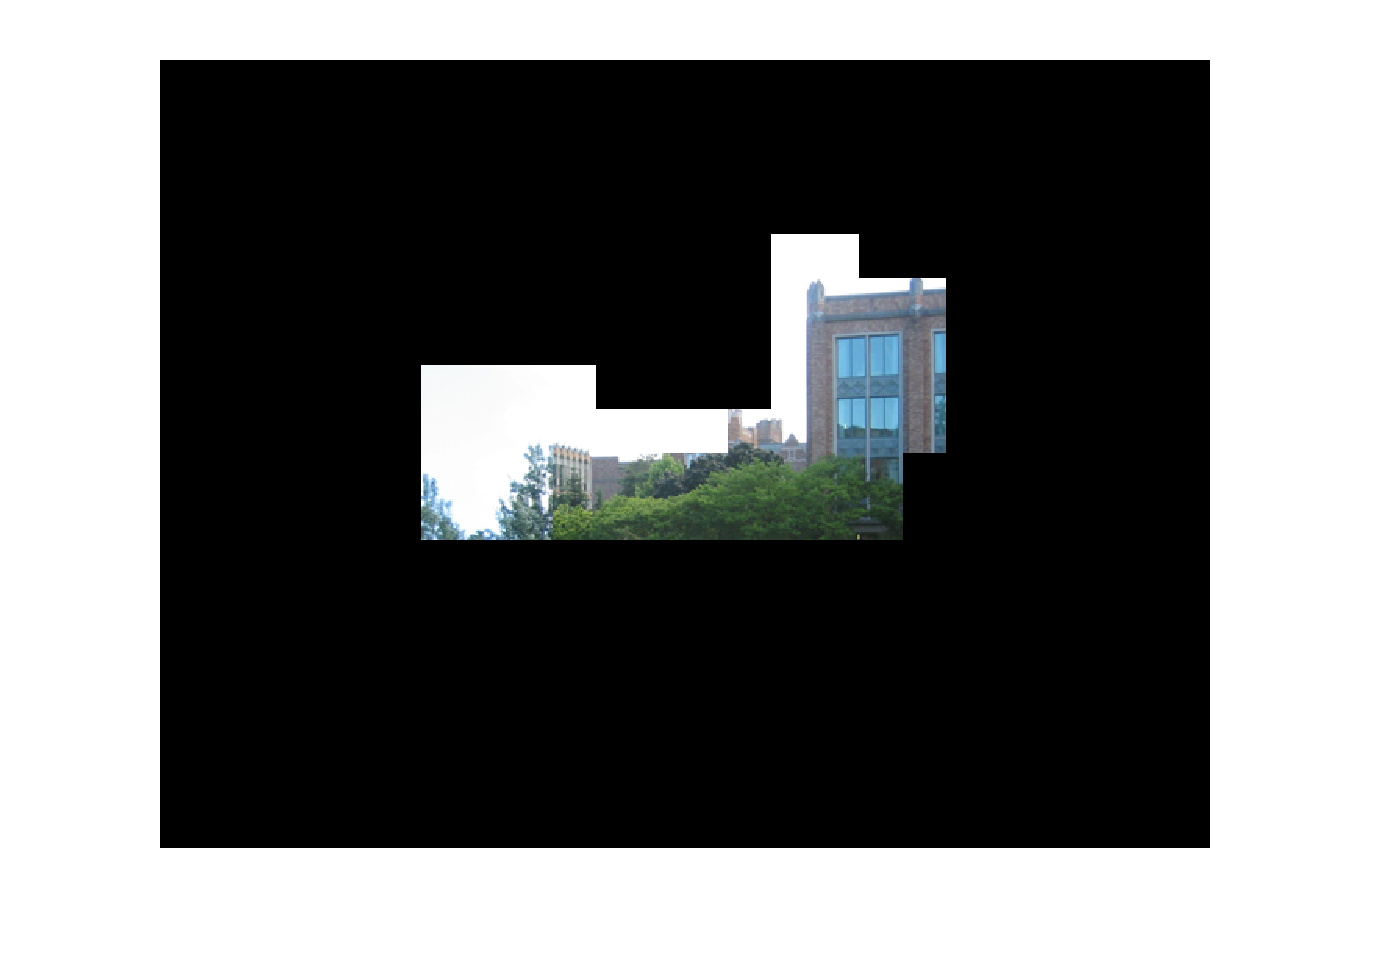
\includegraphics[height=0.25\textheight]{fig/algo_start.eps}
% \label{fig:placement1}}
% \hfil
%     \subfloat[The puzzle is constructed piece by piece.]{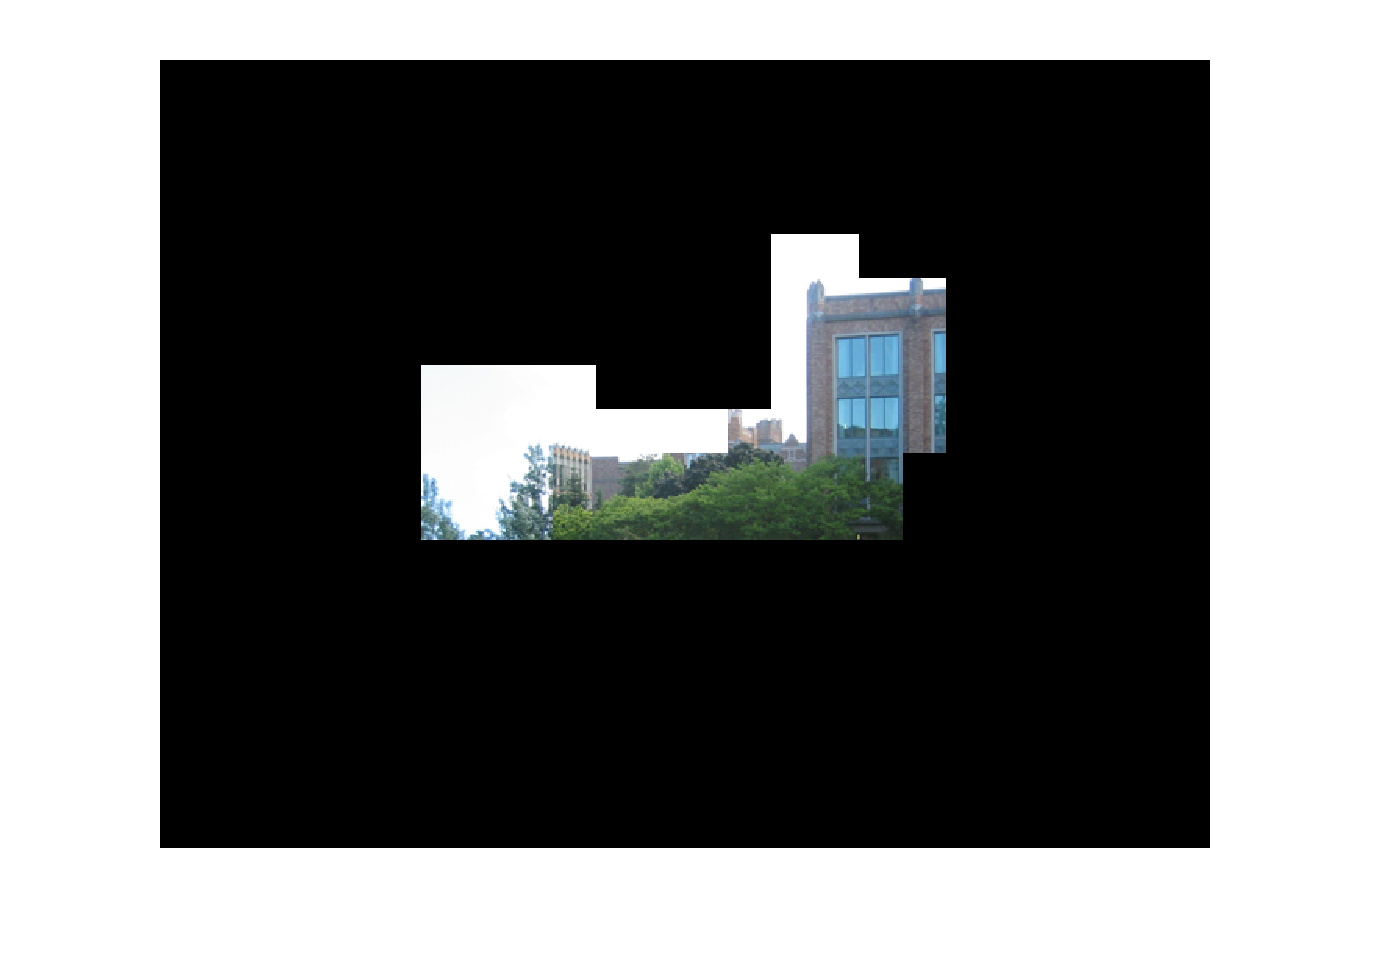
\includegraphics[height=0.25\textheight]{fig/algo_start.eps}
% \label{fig:placement1}}
% \hfil
%     \subfloat[The puzzle is constructed piece by piece.]{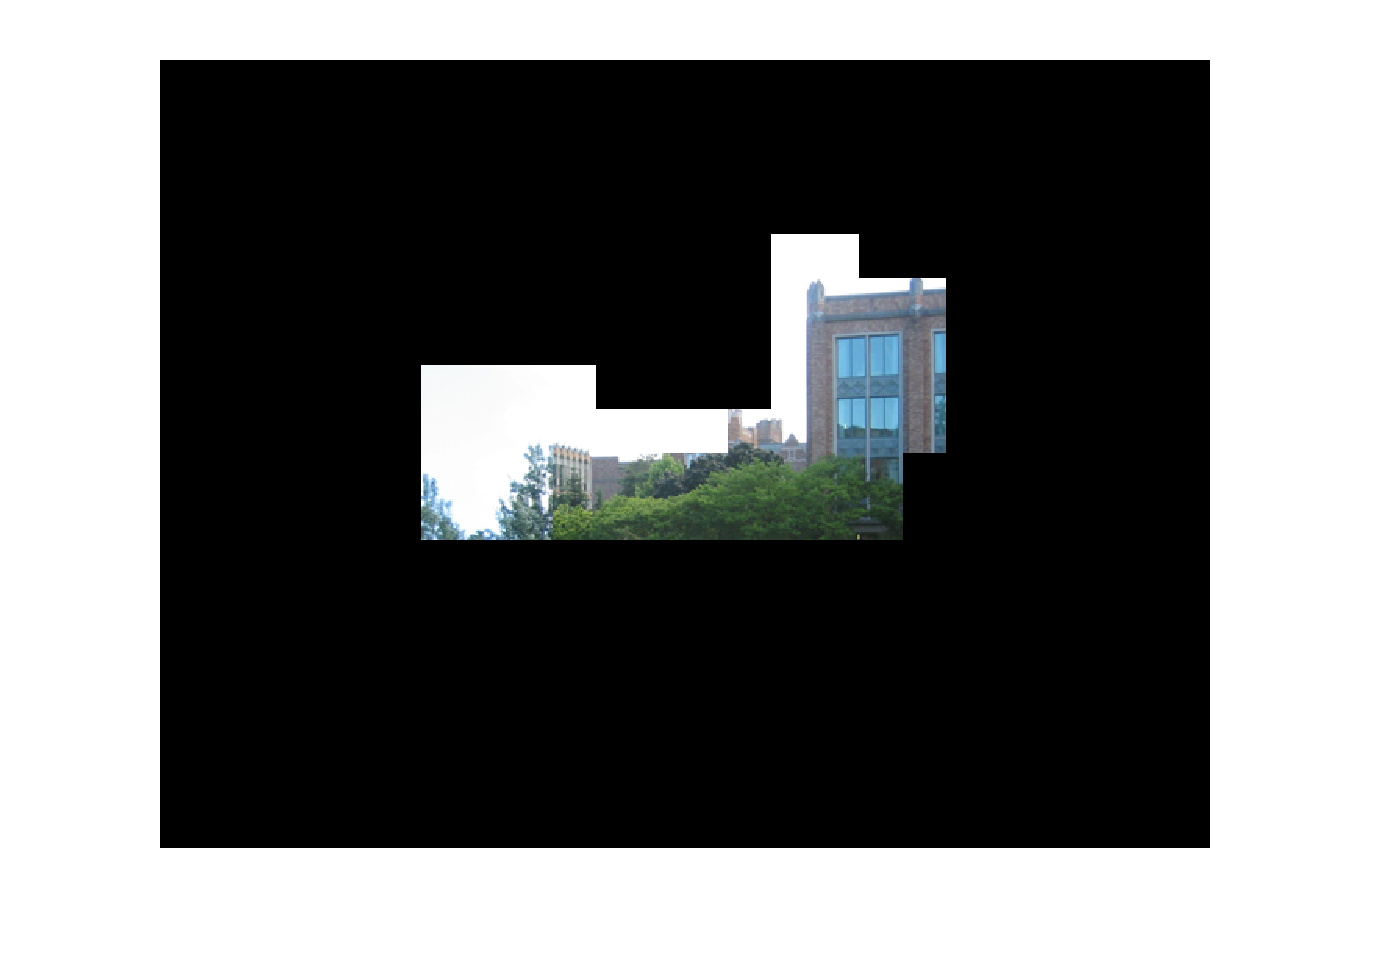
\includegraphics[height=0.25\textheight]{fig/algo_start.eps}
% \label{fig:placement1}}
% \hfil
    \begin{subfigure}{0.25\textheight}
        \centering
        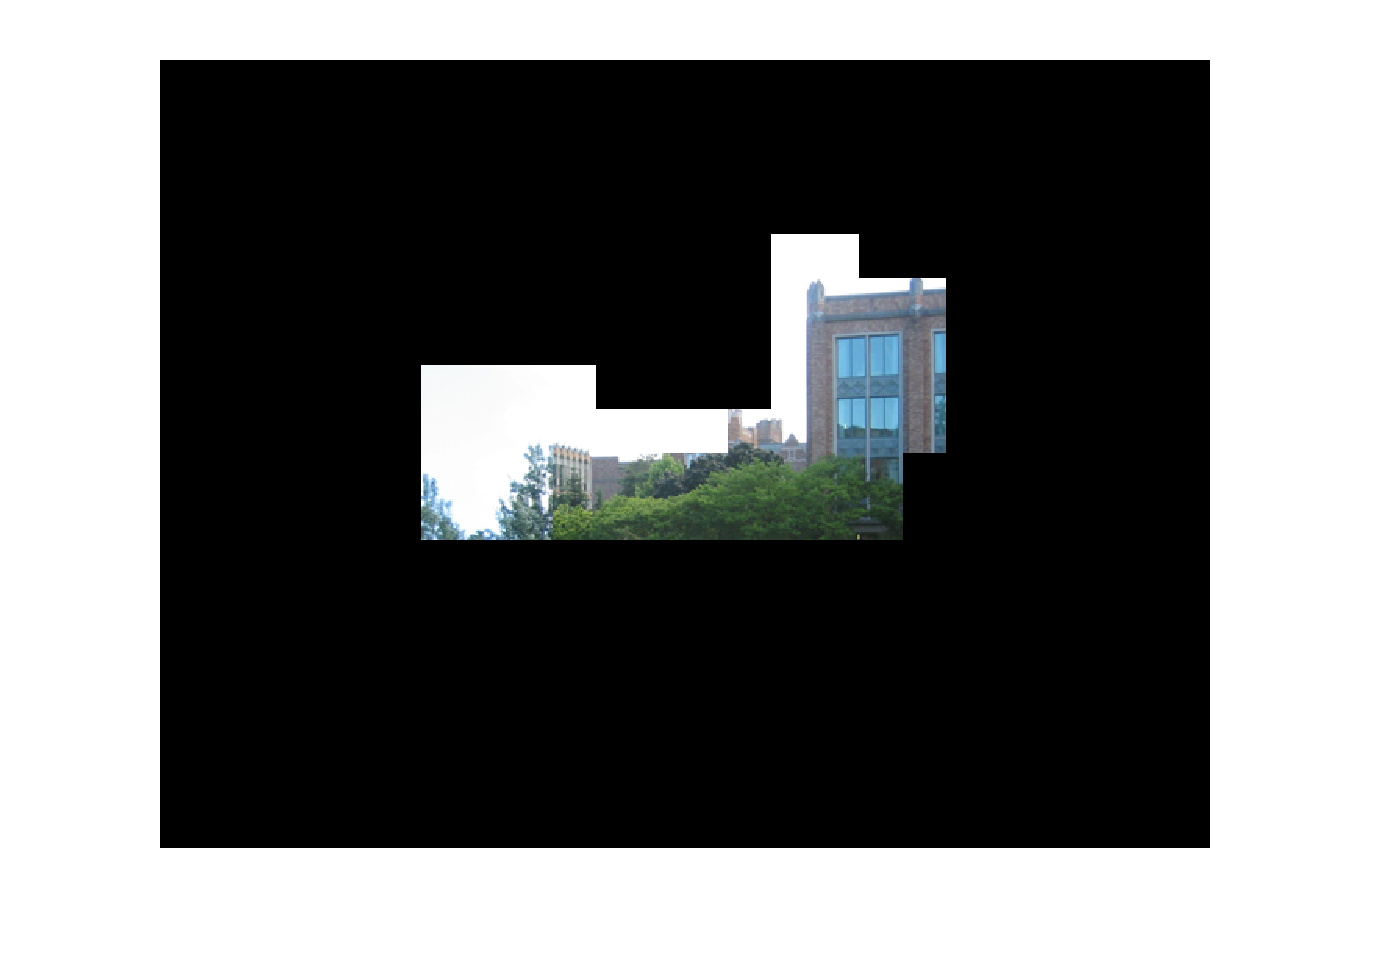
\includegraphics[width=\textwidth]{fig/algo_start.eps}
        \caption{The puzzle is constructed piece by piece.}    
        \label{fig:placement1}
    \end{subfigure}%
    
    \begin{subfigure}[b]{0.25\textheight}
        \centering
        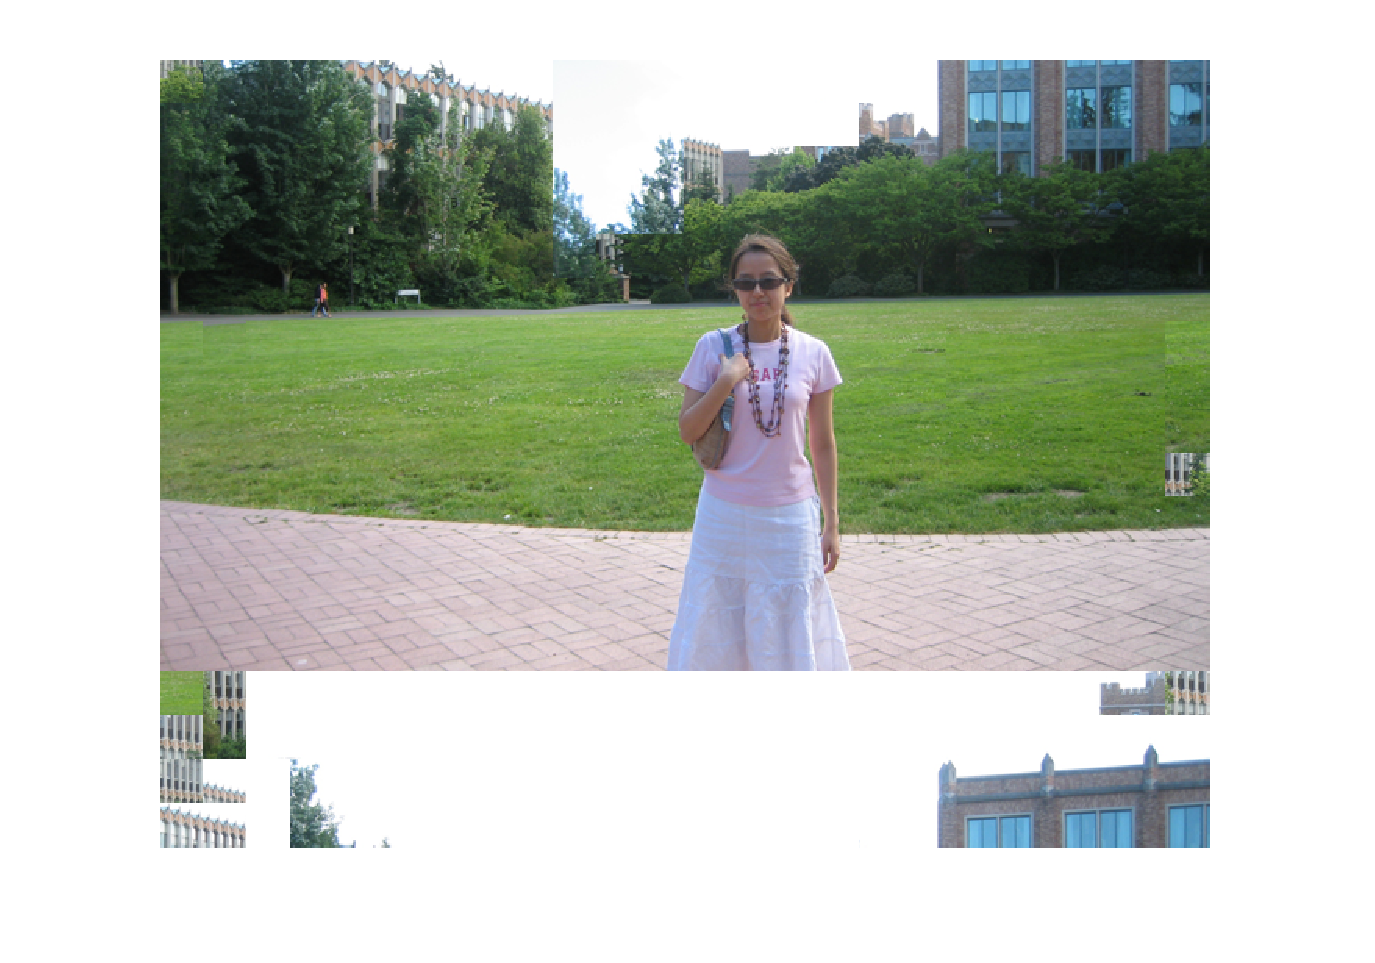
\includegraphics[width=\textwidth]{fig/algo_fin1.eps}
        \caption{At the end of the first placement phase, errors are present.}    
        \label{fig:placement2}
    \end{subfigure}%
    
    \begin{subfigure}[b]{0.25\textheight}
        \centering
        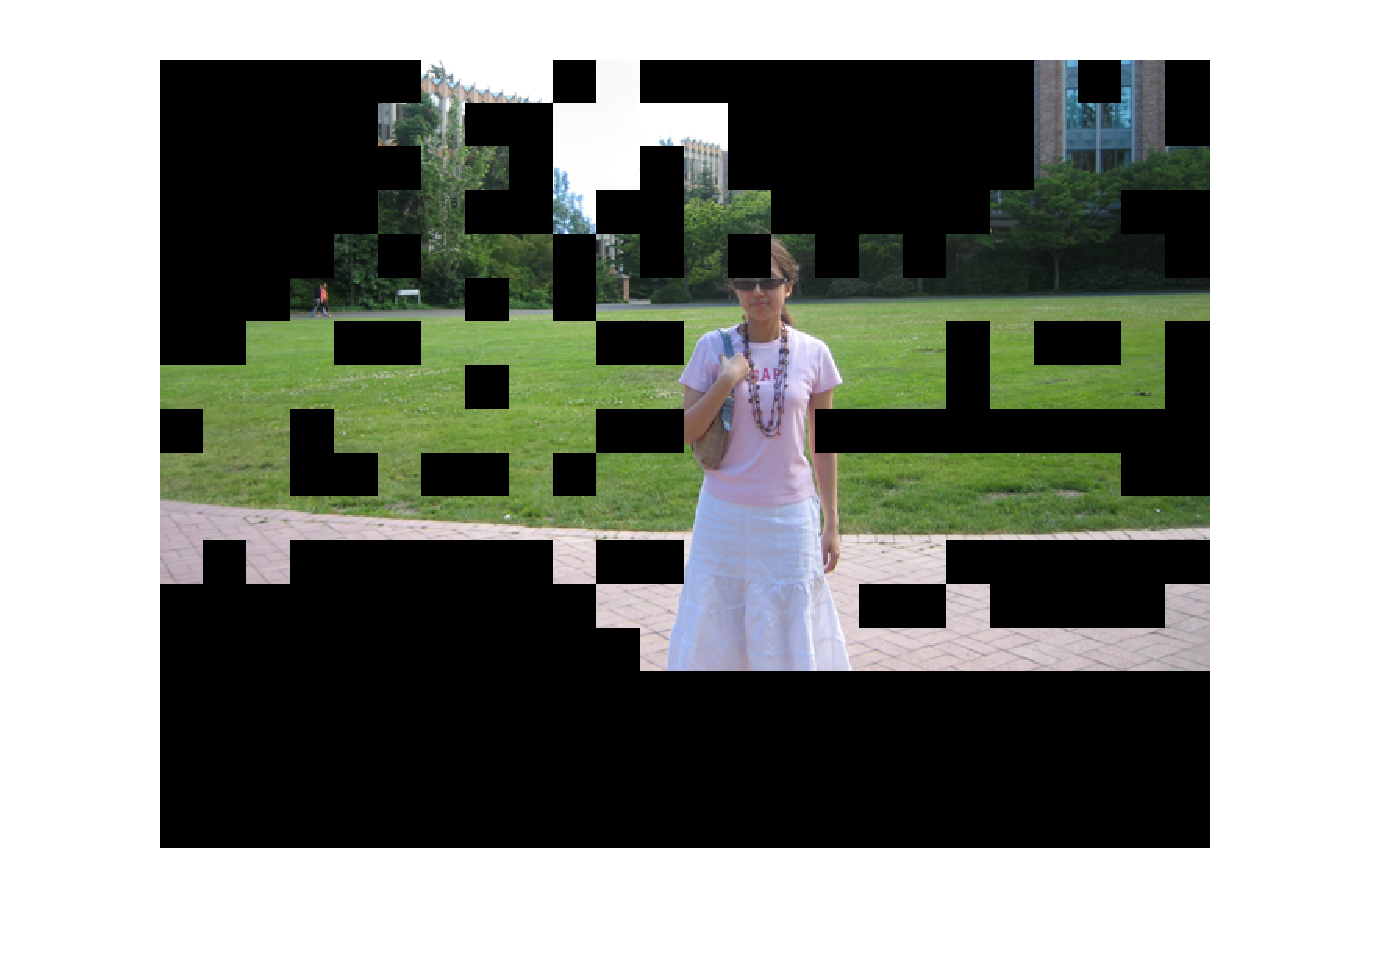
\includegraphics[width=\textwidth]{fig/algo_cut.eps}
        \caption{The biggest segment is extracted from the previous image and will serve as start for the next iteration.}    
        \label{fig:placement3}
    \end{subfigure}%
    
    \begin{subfigure}[b]{0.25\textheight}
        \centering
        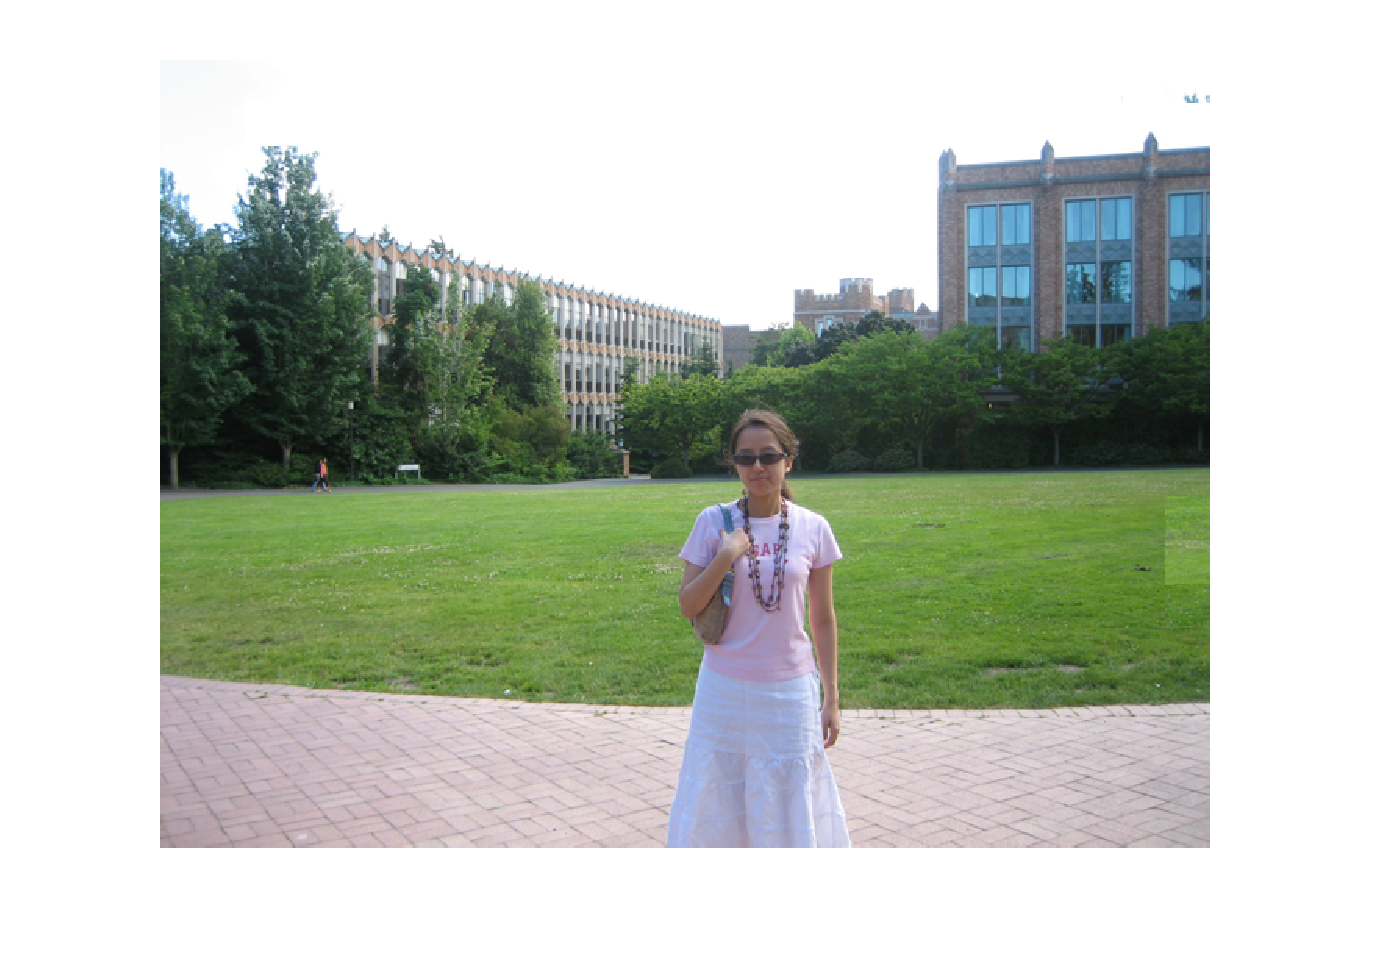
\includegraphics[width=\textwidth]{fig/algo_fin2.eps}
        \caption{The reconstruction is nearly perfect after two iterations.}    
        \label{fig:placement4}
    \end{subfigure}
    
    \caption{Illustration of the reconstruction algorithm}
    \label{fig:placement}
\end{figure}

The Matlab implementation of the algorithm was optimized using matrix computations, and the full solving of a 432 parts puzzle takes less than 10 seconds.